\usepgflibrary{shapes.geometric}
% optical sensor A
\tikzset{
	sensor/.pic={
		\node at (0,.3) {#1};
		\draw (-.2,0.1) rectangle (.2,.2);
		\draw (-.1,0.1) to [out=-90,in=-90] (.1,0.1);
	}
}
\tikzset{
	wedge/.pic={
	\draw[fill=#1] (0,0) -- (1,0) arc [start angle=0,end angle=45,radius=1] -- (0,0);
	}
}
% optical sensor B
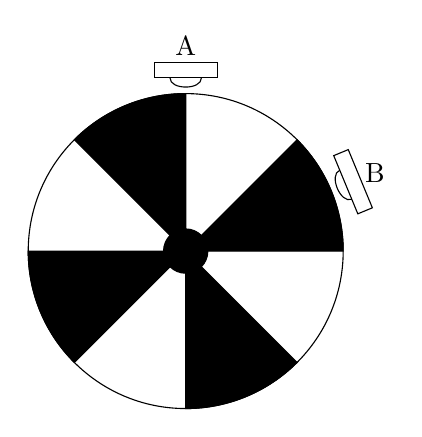
\begin{tikzpicture}[scale=2]
%sensors
\draw (0,1) pic [rotate=0,scale=2] {sensor=A};
\draw (.924,.383) pic [rotate=-67.5,scale=2] {sensor=B};

\draw[fill=white] (0,0) circle[radius=1];
\draw[fill=black] (0,0) circle[radius=0.4em];

\foreach \ang in {0,90,...,270}
	\draw (0,0) pic[rotate=\ang,scale=2] {wedge=black};
\end{tikzpicture}
